In this chapter, we throughly describe the Time Stamped Tries approach
to implement a subsumptive tabling engine. This mechanism was proposed by
Ernie Johnson \textit{et al} \cite{Johnson-99} and is currently implemented in XSB.
It is based on the idea of extending each answer trie node with \textit{timestamp}
information as a means to identify new answers from old answers.

First, we start by describing the algorithms and data structures associated
with the detection of subsuming goals. Next, we explain the data structures
introduced in the answer tries to support subsumption, focusing on answer insertion
and retrieval for subsumed subgoals. Then, we describe the modifications made in the YapTab
tabling engine to support subsumptive tabling. Finally, we compare the performance of
the subsumptive YapTab against XSB, and the variant counterparts.

\section{Finding subsuming goals}

Both DTSA and TSTs use a similar method that given a call trie $C$ and a subgoal $G$
is able to find a subgoal $G'$ that subsumes $G$.

The search is performed by recursively backtracking through the call trie $C$, trying
to match the node symbols with sub-terms or symbols from $G$. The process stops
once a leaf node is reached successfully.

A non-variable symbol from $G$ must only match with an identical symbol from $C$ and
these types of unifications are always tried first.
If the current trie symbol is a variable, for example \texttt{X}, on the first occurrence \texttt{X}
is bound to the respective $G$ sub-term
and match succeeds; on the next occurrences of \texttt{X}, the current sub-term from $G$ must
be identical to the term bound to \texttt{X}. Throughout the backtracking process, bound variables are
always tried before unbound variables.

Favoring constant values before variables, results in a mechanism that finds \textit{minimally subsuming calls}.
Also, if there is some variant call $G''$ in $C$, $G''$ is found before any other subgoal. If no variant 
or no subsuming call are found, it is possible to save the trie node to insert a new variant call.
This trie node is where the first backtracking occurred or when the first occurrence of
an already seen $G$ variable that could not be paired to a bound trie variable, and instead
must be bound to an unbound trie variable for the process to continue.
The new variant path is then used to keep information about the subsumed goal state in
the leaf call trie node.

\begin{figure}[ht]
  \centering
    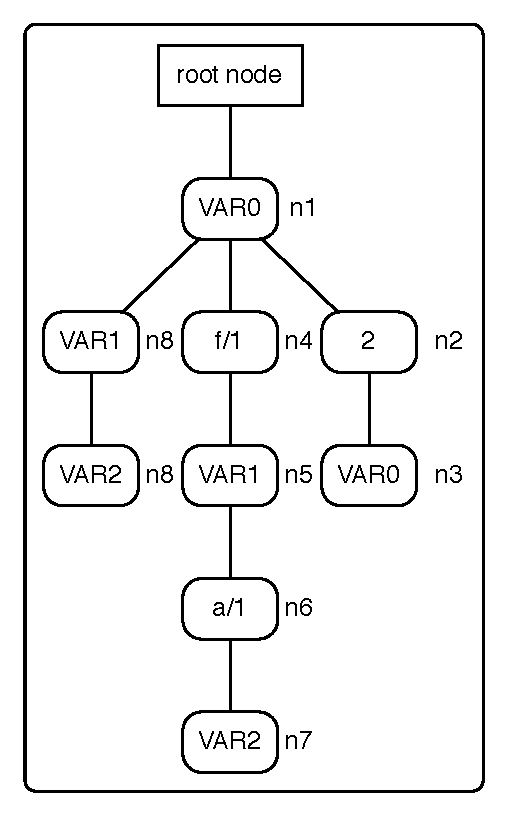
\includegraphics[scale=0.6]{sub_call_search.pdf}
  \caption{Call trie for predicate \texttt{p/3}.}
  \label{fig:sub_call_search}
\end{figure}

For illustration purposes, the Figure \ref{fig:sub_call_search} represents a call trie for the predicate \texttt{p/3}.
The first subgoal called was \texttt{p(X,2,X)}, followed by \texttt{p(X,f(Y),a(Z))} and finally \texttt{p(X,Y,Z)}.

If the subgoal \texttt{p(X,2,X)} is called once again, the algorithm described above
should find the variant subgoal represented by the leaf node $n3$. First, we unify the trie variable
\texttt{VAR0} with \texttt{X} (node $n1$), hence we must also mark the \texttt{X} variable as \textit{seen},
because if the same variable appears again it must unify with the same trie variable for a variant path
to exist. Next, \texttt{2} easily unifies with trie node $n2$ and unification proceeds. In trie node $n3$,
the current call term is \texttt{X} and we also have a variable in the trie node. As \texttt{X} was already seen before,
it must unify with \texttt{VAR0} again, it does and a variant path is found. Please note that if
the trie symbol at node $n3$ was \texttt{VAR1}, the process could proceed but a variant path would be impossible
to exist, and a subsuming subgoal would be found, as \texttt{p(VAR0,2,VAR1)} subsumes \texttt{path(VAR0,2,VAR0)}.
In this case, a variant path could be created by resuming the insert operation at node $n2$ to insert
a \texttt{VAR0} node.

For a more complex example, the subgoal \texttt{p(2,f(X),a(2))} is now called for the same call trie. First,
the algorithm tries to find a trie node with the symbol \texttt{2}, it does not and a variant path
can not be possibly found in this call trie. Next, the algorithm tries to unify with bound variables, but as the process
has just started, only unbound variables can be found and \texttt{VAR0} is unified with \texttt{2} (node $n1$).
The functor term \texttt{f/1} is the next symbol on the subgoal and the first trie node that must be tried is $n4$,
because it contains a non-variable symbol. The next term is \texttt{X} and it can unify with \texttt{VAR1} (node $n5$).
Next, the term symbol \texttt{a/1} matches with trie node $n6$ and the process proceeds. Note that if we failed
at this point, the process would backtrack to node $n2$ and node $n8$ would be tried next, which would
lead to a more general subgoal. Back to node $n6$, the last term symbol \texttt{2} can match with node $n7$, as it is the only trie
node available and it is an unbound variable. If the variable was bound, like \texttt{VAR0} for instance,
the process would check if the current term symbol unifies with the variable binding made before (\texttt{VAR0 = 2}) and
it would also succeed. As node $n7$ is a leaf node, the process finishes and a subsumptive path is found.
The following variable bindings were made: \texttt{VAR0 = 2}, \texttt{VAR1 = X}, and \texttt{VAR2 = 2}.

\subsection{Implementation details}

This algorithm uses various data structures: three auxiliary stacks, a call choice point stack,
a variable bindings vector, and variable enumerator vector. The following summarizes
each data structure: 

\begin{itemize}
  \item \textit{variable bindings vector}: saves bindings for each numbered trie variable. Starts with each position pointing to itself;
  \item \textit{variable enumerator vector}: when a never seen term variable appears it must be bound to a position in this enumerator, ensuring that it can be recognized if it appears a second time;
  \item \textit{term stack}: stores the remaining terms to be unified against trie symbols;
  \item \textit{term log stack}: stores the already matched terms. Each frame contains the top index and the top element of the term stack during frame's creation;
  \item \textit{trail stack}: stores bindings that were made during the process. It is used to untrail variables during backtracking;
  \item \textit{call choice point stack}: used to restore the search process at a certain node to explore alternatives.
\end{itemize}

During execution, two matching methods are considered: the first tries to match exact trie symbols against the current term;
the second method uses trie variables instead of exact symbols and is employed when the first method fails.
When a trie node match succeeds, matching defaults to the first method, which means
that exact matches are always tried before variables when a new \textit{trie level} is reached and variables are mainly
used when backtracking. A trie level represents a set of nodes that are linked by \texttt{sibling} links or are at
the same hash table.

\begin{figure}[ht]
  \centering
    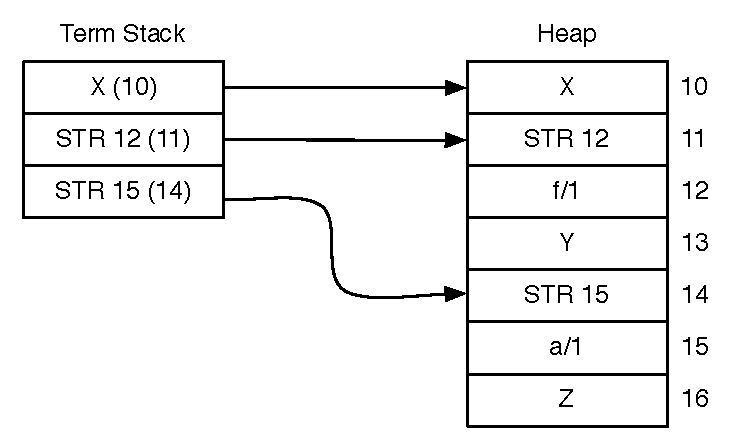
\includegraphics[scale=0.6]{lookup_subgoal_termstack_start.pdf}
  \caption{Initial term stack and heap for subgoal \texttt{p(X,f(Y),a(Z))}.}
  \label{fig:lookup_subgoal_termstack_start}
\end{figure}

The process starts by pushing the $G$ subgoal arguments, $X1, X2, ...Xn$ into the term stack, so that $X1$ is at the top
and $Xn$ at the bottom (Figure \ref{fig:lookup_subgoal_termstack_start}).
Then, the algorithm proceeds in a modified depth-first manner, trying to match the exact nodes first, and then
the variable trie nodes. The skeleton for this algorithm is presented in Figure \ref{fig:lookup_subsuming_call}.

\begin{figure}[ht]
\begin{Verbatim}[fontsize=\small]
lookup_subsuming_call(call_trie) {
  match_mode = MATCH_EXACTLY
  parent = trie_root(call_trie)
  node = child(parent)
  variable_chain = NULL

while_loop:
  while(termstack is not empty) {
    subterm = deref(termstack_pop())
    termstacklog_push(termstack_index(), termstack_top())
  
    if(subterm is atom or integer)
      match_constant(subterm)
    else if(subterm is functor or list)
      match_structured_term(subterm)
    else if(subterm is variable)
      match_variable(subterm)
  
    if(current match failed)
      if(choice point stack is empty) // no more alternatives
        return NO_PATH
      else
        (alt_node, var_chain) = ccpstack_pop_frame()
        match_mode = MATCH_TRIE_VARS
  }
}
\end{Verbatim}
\caption{Pseudo\-code for \texttt{lookup\_subsuming\_call}.}
\label{fig:lookup_subsuming_call}
\end{figure}

\subsubsection{Call choice point stack}

The call choice point stack (Figure \ref{fig:call_choice_point_stack}) contains alternative
search paths to use if the process fails somewhere in the trie.
Each stack frame can restore the search at a given node by restoring all the auxiliary stacks state at the time
of the call frame creation.

\begin{figure}[ht]
  \centering
    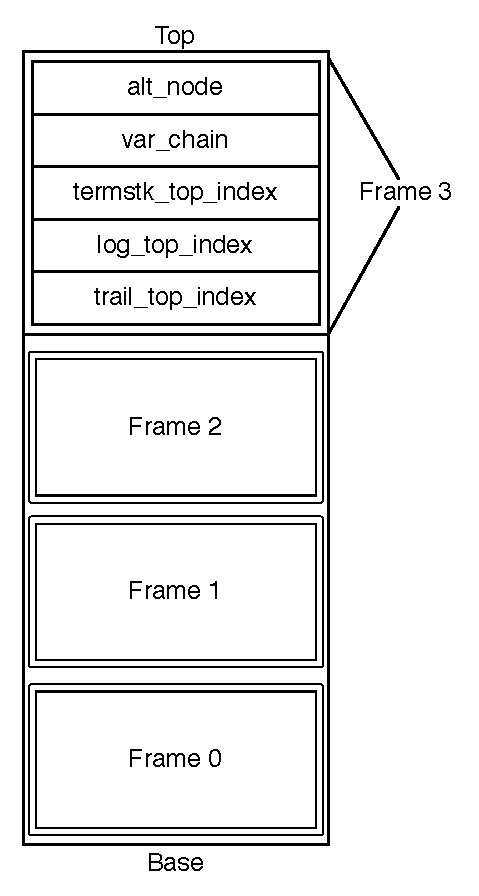
\includegraphics[scale=0.6]{call_choice_point_stack.pdf}
  \caption{Call choice point stack organization.}
  \label{fig:call_choice_point_stack}
\end{figure}

Each frame contains the next trie node to explore (\texttt{alt\_node}),
the current variable chain (\texttt{var\_chain}),
and the following stack indexes during frame creation:
the top of the term stack (\texttt{termstk\_top\_index}),
the top of the term log stack (\texttt{log\_top\_index}),
and the top of the trail stack (\texttt{trail\_top\_index}).
The function \texttt{ccpstack\_push\_frame} (Figure \ref{fig:ccpstack_push_frame})
is used to create a new frame from the computation state.

\begin{figure}[ht]
\begin{Verbatim}[fontsize=\small]
ccpstack_push_frame(alt_node, var_chain) {
  CCPFrame new_frame = new CPPFrame()
  new_frame.alt_node = alt_node
  new_frame.var_chain = var_chain
  new_frame.termstk_top_index = termstack_top - termstack_base + 1
  new_frame.log_top_index = termstacklog_top - termstacklog_base - 1
  new_frame.trail_top_index = trail_top - trail_base
  ccpstack_push(new_frame)
}
\end{Verbatim}
\caption{Pseudo\-code for \texttt{ccpstack\_push\_frame}.}
\label{fig:ccpstack_push_frame}
\end{figure}

When popping a frame from the stack, the state of the auxiliary stacks and the other data
structures is restored. Consider a computational state $S1$ that pushed unto the stack
the frame $F1$. Given that we are at state $S2$ and we need to backtrack to the previous state, $S1$,
first we need remove $F1$ from the stack and use the frame's information to restore $S1$.

Any terms that were popped from the term stack from $S1$ to $S2$, which were
stored in the term log stack must be restored back into the term stack.
Then, any bindings made from $S1$ to $S2$ must be untrailed, which is
accomplished by \textit{unwinding} the trail stack. The unwind process untrails
any trie variables bound to the trie variable bindings vector
and any term variable which may have been made to point to the variable enumerator. 

Finally the alternative node and
the variable chain at state $S1$ is also restored. All this is accomplished by the
function \texttt{ccpstack\_pop\_frame} (Figure \ref{fig:ccpstack_pop_frame}).

\begin{figure}[h]
\begin{Verbatim}[fontsize=\small]
ccpstack_pop_frame() {
  CCPFrame top_frame = ccpstack_pop()
  termstacklog_unwind(top_frame.log_top_index)
  termstack_set_top_of_stack(top_frame.termstk_top_index)
  trail_unwind(top_frame.trail_top_index)
  
  return (top_frame.alt_node, top_frame.var_chain)
}
\end{Verbatim}
\caption{Pseudo\-code for \texttt{ccpstack\_push\_frame}.}
\label{fig:ccpstack_pop_frame}
\end{figure}

The node associated with $S2$ and its successors are never visited again and
the process continues until a leaf node is reached or the call choice point stack
is exhausted and the entire trie is visited, yielding no results.

\subsubsection{Matching constants}

The \texttt{match\_constant} function is called when the next term from the term stack is a integer or an
atom. First, in phase \textbf{(1)}, the function checks if the match method is to exactly match the
subterm constant against a trie symbol, which means
that this is the first time this trie level is explored. If the current trie level is represented by a simple
linked list, both \texttt{node} and \texttt{var\_chain} point to the start of the chain, but if the trie level
is an hash table, \texttt{node} will point to the symbol bucket and \texttt{var\_chain} to the variable
bucket, which usually is the first bucket.

\begin{figure}[h]
\begin{Verbatim}[fontsize=\small]
match_constant(constant) {
  if match_mode == MATCH_EXACTLY // (1)
    (node, var_chain) = set_node_and_var_chain(constant)
    match_node = find_matching_node(constant, node)
    if match_node is not NULL
      conditionally_create_choice_point(var_chain)
      descend_node(match_node)
    else // no match found
      node = var_chain
      no_variant_found(parent)
  // no exact match, try bound trie variables (2)
  match_node = find_bound_trie_var(constant, node)
  if match_node is not NULL
    ccpstack_push_frame(next(match_node), var_chain)
    descend_node(match_node)
  // no bound trie variable found, use unbound trie variables (3)
  match_node = find_unbound_trie_var(var_chain)
  if match_node is not NULL
    bind_trie_var(match_node, constant)
    descend_node(match_node)
}
\end{Verbatim}
\caption{Pseudo\-code for \texttt{match\_constant}.}
\label{fig:match_constant}
\end{figure}

The function \texttt{find\_matching\_node} iterates a linked list and locates a trie node that contains the
\texttt{constant} symbol. If this node is found we conditionally create a
new choice point (Figure \ref{fig:conditionally_create_choice_point}), that is
we try to find a node with a variable that can be used when backtracking. At this point, only
trie variables can be explored as only one node with the matched symbol exists at this level.

\begin{figure}[ht]
\begin{Verbatim}[fontsize=\small]
conditionally_create_choice_point(var_chain) {
  foreach(node in var_chain)
    if(is_trie_var(node))
      ccpstack_push_frame(node, node)
      return
}
\end{Verbatim}
\caption{Pseudo\-code for \texttt{conditionally\_create\_choice\_point}.}
\label{fig:conditionally_create_choice_point}
\end{figure}

Please note that the found variable node is used as the alternative node in this choice point
and as the variable chain, which will be used to try bound and unbound trie nodes, when backtracking happens.

To descend into a node when a matching succeeds the function \texttt{descend\_node} (Figure \ref{fig:descend_node})
is used. It sets the current \texttt{node} and \texttt{parent} information, sets the matching mode for a new trie level
and changes the program flow to the main \texttt{lookup\_subsuming\_call} while loop. But,
if an exact match fails, we know that the current path cannot be variant of the called subgoal, and we call
\texttt{no\_variant\_found} with the parent node as argument.

\begin{figure}[ht]
\begin{Verbatim}[fontsize=\small]
descend_node(target_node) {
  parent = target_node
  node = child(target_node)
  match_mode = MATCH_EXACTLY
  goto while_loop
}
\end{Verbatim}
\caption{Pseudo\-code for \texttt{descend\_node}.}
\label{fig:descend_node}
\end{figure}

Phase \textbf{(2)} of \texttt{match\_constant} can be reached by a failed exact match or by backtracking
(remember that the match mode changes to \texttt{MATCH\_TRIE\_VARS} when backtracking). In this step
we call \texttt{find\_bound\_trie\_var} that will iterate over the \texttt{node} chain to look for
\textit{bound trie variables}. When inserting new subgoals on the call trie, each new trie variable
along a path is marked, so it is easy to check for old variables, which have already been bound
to some term before arriving at the current node. The variable binding can be retrieved by
checking the trie variable bindings position for this variable number, which points to an heap term.
Given that we are trying to match a constant symbol, we verify if the bound term matches our symbol.
In this case, we create a new choice point for the sibling node of the matched trie variable, and use
the currently set variable chain.

Finally, if phase \textbf{(1)} and \textbf{(2)} fail, we try to match our constant against an unbound trie variable
(Figure \ref{fig:find_unbound_trie_var}).
Phase \textbf{(3)} can be also reached by a failed exact and bound trie variable match or by subsequent backtrack
attempts. If a node is found, we bind the variable position on the trie variable bindings
vector to point to the new constant. This position is also trailed on the trail stack, so that it can be untrailed
if backtracking is executed.

\begin{figure}[ht]
\begin{Verbatim}[fontsize=\small]
find_unbound_trie_var(var_chain) {
  foreach(node in var_chain)
    if(is_variable(node) and is_new_variable(node))
      return node
}
\end{Verbatim}
\caption{Pseudo\-code for \texttt{find\_unbound\_trie\_var}.}
\label{fig:find_unbound_trie_var}
\end{figure}

\subsubsection{Matching structured terms}

When a structured term appears on the term stack, either a functor or a list, the matching process works
just like constants, except the functor or list arguments must be pushed unto the term stack after an exact
match is found (Figure \ref{fig:match_structured_term}).

\begin{figure}[h]
\begin{Verbatim}[fontsize=\small]
match_structured_term(term) {
  if match_mode == MATCH_EXACTLY // (1)
    (node, var_chain) = set_node_and_var_chain(term)
    match_node = find_matching_node(term, node)
    if match_node is not NULL
      termstack_push_arguments(term)
      conditionally_create_choice_point(var_chain)
      descend_node(match_node)
    else // no match found
      node = var_chain
      no_variant_found(parent)
  // no exact match, try bound trie variables (2)
  match_node = find_bound_trie_var(term, node)
  if match_node is not NULL
    ccpstack_push_frame(next(match_node), var_chain)
    descend_node(match_node)
  // no bound trie variable found, use unbound trie variables (3)
  match_node = find_unbound_trie_var(var_chain)
  if match_node is not NULL
    bind_trie_var(match_node, term)
    descend_node(match_node)
}
\end{Verbatim}
\caption{Pseudo\-code for \texttt{match\_structured\_term}.}
\label{fig:match_structured_term}
\end{figure}

Figure \ref{fig:match_functor} shows the evolution of the term stack for finding
a subsuming goal for the subgoal \texttt{p(a,f(b))}. Step \textbf{(1)} shows the initial 
term stack, followed by a match of the term on top of the stack, \texttt{a}, against \textbf{VAR0}.
As it is an unbound trie variable, the first position of the variable bindings vector is
bound to the target term, \texttt{a}.
In step \textbf{(2)}, we try to match the functor \texttt{f/1} against node \textbf{(b)}, but we fail.
Node \textbf{(c)} succeeds as it is an exact match and the functor argument, \texttt{b}, is pushed on
the term stack. In step \textbf{(3)}, \texttt{b} matches against \texttt{b}, and we find a subsuming call:
\texttt{p(VAR0,f(b))}.

\begin{figure}[ht]
  \centering
    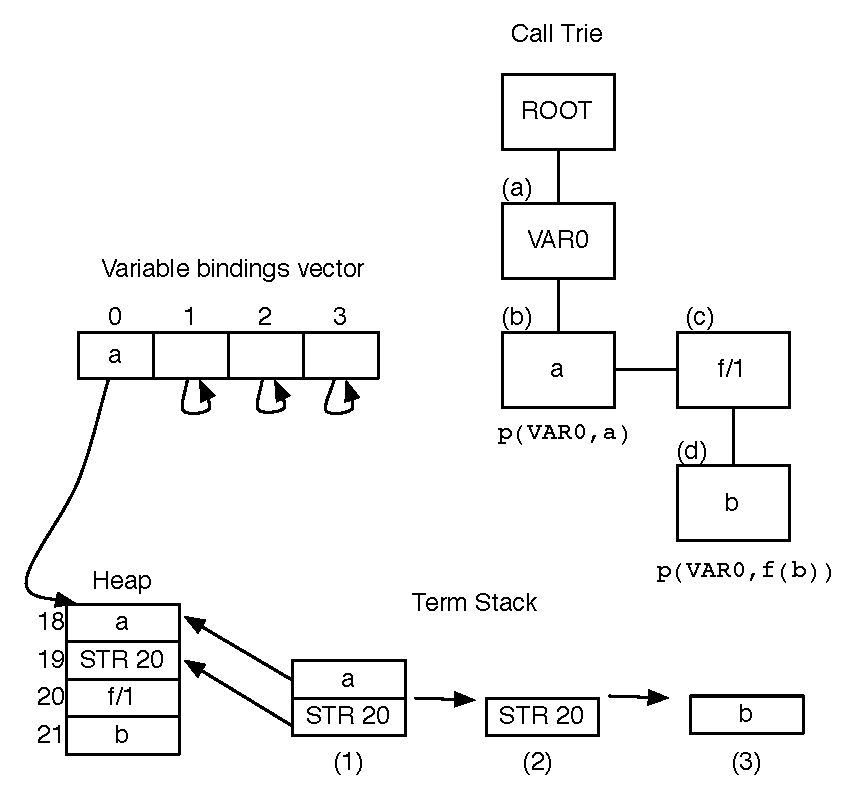
\includegraphics[scale=0.6]{match_functor.pdf}
  \caption{Finding a subsuming goal for subgoal \texttt{p(a,f(b))}.}
  \label{fig:match_functor}
\end{figure}

\subsubsection{Matching variables}

The last case for matching terms are variables. Because we are trying to find a more general goal,
a term variable must only be matched or bound against a trie variable and nothing else. More, a
never seen variable must match only with an unbound trie variable, consider the case of trying to
match \texttt{p(X,Y)} against \texttt{p(X,X)}, the first call variable could match the first trie variable,
but the call variable \texttt{Y} must be matched against an unbound variable, thus the next trie variable
(in this case \texttt{VAR0}) cannot be matched, because it was already bound to another variable.
Please note that \texttt{p(X,X)} is subsumed by \texttt{p(X,Y)} and not the other way around.

To recognize already seen call variables, we bind them to the variable enumerator array, indexed
by the corresponding trie variable number and use the trail stack to trail them.
When such call variable must be matched again with a
trie variable, we first try to match it with the same trie variable, and if we fail to find such trie
variable, we use an unbound trie variable, thus, we avoid binding two different call variables to the same
trie variable.

\begin{figure}[h]
\begin{Verbatim}[fontsize=\small]
match_variable(term) { // term represents a variable on the heap
  if match_mode == MATCH_EXACTLY
    if node is not NULL and is_hash_table(node)
      node = var_chain = hash_bucket(node, VARIABLE_BUCKET)
    else
      var_chain = node
    if variable is not marked(term)
      // variable not seen before
      // only one new trie variable per level, no choice point needed
      foreach(test_node in node) {
        if is_trie_var(test_node) and is_new_variable(test_node)
          bind_trie_var(test_node, term)
          mark_prolog_var(term, var_index(test_node))
          descend_node(test_node)
      no_variant_found(parent)
      backtrack
  // variable has been seen before
  foreach(test_node in node)
    if is_trie_var(test_node) and !is_new_variable(test_node)
      if identical_terms(trie_var_bindings[test_node], term)
        ccpstack_push_frame(next(test_node), var_chain)
        descend_node(test_node)
  // variant path is not possible here
  no_variant_found(parent)
  // match against unbound trie variable
  foreach(test_node in var_chain)
    // only one new trie variable per level, no choice point needed
    if is_trie_var(test_node) and is_new_variable(test_node)
      bind_trie_var(test_node, trie_var_bindings[prolog_var_index(term)])
      descend_node(test_node)
}
\end{Verbatim}
\caption{Pseudo\-code for \texttt{match\_variable}.}
\label{fig:match_variable}
\end{figure}

The pseudo-code to match against a variable is displayed in Figure
\ref{fig:match_variable}. From it, we can conclude that a variant path
cannot be found when: (1) a new trie variable cannot be found
for a new call variable, (2) we cannot match an already seen
call variable against the same trie variable already bound to it.

\subsubsection{Variant continuations}

\section{Answer Templates}

\section{Answer Insertion on TSTs}

\section{Collecting Relevant Answers}

\section{Consuming Answers}

\section{Compiled Tries}

\section{Subsumptive YapTab}

\section{Results}